\documentclass[border=2pt]{standalone}
\usepackage{tikz}
\usepackage{amsmath}
\begin{document}
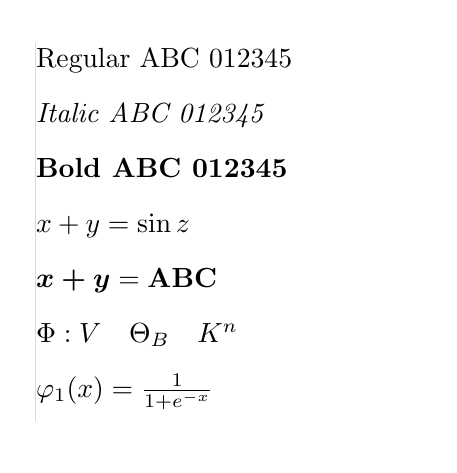
\begin{tikzpicture}
  \path[use as bounding box] (-.1,.5) rectangle (5,-4.8);
  \draw[gray!30,thin] (0,.3) -- (0,-4.5);
  \node[anchor=base west,inner sep=0pt] at (0,0) {Regular ABC 012345};
  \node[anchor=base west,inner sep=0pt,font=\itshape] at (0,-.7) {Italic ABC 012345};
  \node[anchor=base west,inner sep=0pt,font=\bfseries] at (0,-1.4) {Bold ABC 012345};
  \node[anchor=base west,inner sep=0pt] at (0,-2.1) {$x+y=\sin z$};
  \node[anchor=base west,inner sep=0pt] at (0,-2.8) {$\boldsymbol{x+y}=\mathbf{ABC}$};
  \node[anchor=base west,inner sep=0pt] at (0,-3.5) {$\Phi:V\quad\Theta_B\quad K^n$};
  \node[anchor=base west,inner sep=0pt] at (0,-4.2) {$\varphi_1(x)=\frac{1}{1+e^{-x}}$};
\end{tikzpicture}
\end{document}
